% Guía de uso del trabajo. Compilar (desde esta carpeta):   tectonic -X compile guia_de_uso.tex
\documentclass[11pt,a4paper,twoside,openany]{report}
% Preámbulo común de la memoria y de la guía de uso.
% Tipografía: Libertinus (texto y matemáticas), cuerpo 11 pt, interlineado holgado. Compilar con Tectonic o XeLaTeX.

\usepackage[spanish,es-noshorthands,es-tabla,es-nodecimaldot]{babel}
\usepackage{libertinus}
\usepackage{microtype}
\usepackage[a4paper,top=2.7cm,bottom=2.7cm,inner=2.8cm,outer=2.4cm,headheight=15pt]{geometry}
\linespread{1.13}
\clubpenalty=10000
\widowpenalty=10000
\displaywidowpenalty=10000
\raggedbottom
\emergencystretch=2.5em
\tolerance=1200
\hbadness=3000

\usepackage{amsmath}
\usepackage{etoolbox}
\usepackage{xcolor}
\usepackage{graphicx}
\usepackage{placeins}
\usepackage{float}
\usepackage{caption}
\usepackage{subcaption}
\usepackage{booktabs,tabularx,array,multirow,makecell}
\usepackage{enumitem}
\usepackage{needspace}
\usepackage{fancyhdr}
\usepackage{titlesec}
\usepackage{listings}
\usepackage{tikz}
\usetikzlibrary{arrows.meta,positioning,shapes.geometric,fit,calc}
\usepackage{algorithm}
\usepackage{algpseudocode}
\usepackage[hidelinks,bookmarksnumbered]{hyperref}

% ── Colores (los mismos de las figuras y de la web) ──
\definecolor{azul}{HTML}{2A78D6}
\definecolor{naranja}{HTML}{EB6834}
\definecolor{aqua}{HTML}{1BAF7A}
\definecolor{amarillo}{HTML}{EDA100}
\definecolor{rosa}{HTML}{E87BA4}
\definecolor{verde}{HTML}{008300}
\definecolor{violeta}{HTML}{6250D6}
\definecolor{rojo}{HTML}{E34948}
\definecolor{gris}{HTML}{52514E}
\definecolor{grisclaro}{HTML}{F1F0EC}
\definecolor{tinta}{HTML}{14203A}

% ── Títulos: cada capítulo empieza en página nueva; los apartados no se quedan huérfanos al pie de la página ──
\titleformat{\chapter}[display]{\normalfont\bfseries\color{tinta}}{\large\scshape\color{gris}Capítulo \thechapter}{0.35em}{\Huge}[\vspace{0.4em}\titlerule]
\titlespacing*{\chapter}{0pt}{-10pt}{26pt}
\titleformat{\section}{\normalfont\Large\bfseries\color{tinta}}{\thesection}{0.7em}{}
\titlespacing*{\section}{0pt}{2.0ex plus 0.4ex}{1.1ex plus 0.2ex}
\titleformat{\subsection}{\normalfont\large\bfseries\color{tinta}}{\thesubsection}{0.7em}{}
\titlespacing*{\subsection}{0pt}{1.7ex plus 0.3ex}{0.8ex plus 0.2ex}
\titleformat{\subsubsection}{\normalfont\normalsize\bfseries\itshape\color{gris}}{}{0pt}{}
\titlespacing*{\subsubsection}{0pt}{1.3ex plus 0.2ex}{0.5ex plus 0.1ex}
% Si queda menos de ~28 % de página, el apartado empieza en la página siguiente (así no se parte por la mitad)
\pretocmd{\chapter}{\FloatBarrier}{}{}
\pretocmd{\section}{\Needspace{0.40\textheight}}{}{}
\pretocmd{\subsection}{\Needspace{0.22\textheight}}{}{}
\pretocmd{\subsubsection}{\Needspace{0.10\textheight}}{}{}

% ── Cabecera y pie ──
\pagestyle{fancy}
\fancyhf{}
\fancyhead[LE]{\small\slshape\leftmark}
\fancyhead[RO]{\small\slshape\rightmark}
\fancyfoot[C]{\small\thepage}
\renewcommand{\headrulewidth}{0.3pt}
\renewcommand{\chaptermark}[1]{\markboth{#1}{}}
\renewcommand{\sectionmark}[1]{\markright{\thesection\ \ #1}}
\fancypagestyle{plain}{\fancyhf{}\fancyfoot[C]{\small\thepage}\renewcommand{\headrulewidth}{0pt}}

% ── Figuras, tablas y listas ──
\captionsetup{font=small,labelfont=bf,labelsep=period,justification=centering,format=plain}
\captionsetup[table]{position=above,skip=6pt}
\captionsetup[figure]{position=below,skip=6pt}
\setlist{itemsep=0.25em,topsep=0.4em,parsep=0pt}
\renewcommand{\arraystretch}{1.18}
\graphicspath{{figuras/}{../web/capturas/}{capturas/}}
\renewcommand{\topfraction}{0.88}\renewcommand{\bottomfraction}{0.7}\renewcommand{\textfraction}{0.12}\renewcommand{\floatpagefraction}{0.65}\setcounter{topnumber}{3}\setcounter{totalnumber}{5}
\setcounter{tocdepth}{2}
\setcounter{secnumdepth}{3}

% ── Pseudocódigo en español ──
\floatname{algorithm}{Algoritmo}
\renewcommand{\listalgorithmname}{Lista de algoritmos}
\algrenewcommand\algorithmicrequire{\textbf{Entrada:}}
\algrenewcommand\algorithmicensure{\textbf{Salida:}}
\algrenewcommand\algorithmicwhile{\textbf{mientras}}
\algrenewcommand\algorithmicdo{\textbf{hacer}}
\algrenewcommand\algorithmicfor{\textbf{para}}
\algrenewcommand\algorithmicforall{\textbf{para cada}}
\algrenewcommand\algorithmicif{\textbf{si}}
\algrenewcommand\algorithmicthen{\textbf{entonces}}
\algrenewcommand\algorithmicelse{\textbf{si no}}
\algrenewcommand\algorithmicrepeat{\textbf{repetir}}
\algrenewcommand\algorithmicuntil{\textbf{hasta que}}
\algrenewcommand\algorithmicreturn{\textbf{devolver}}
\algrenewtext{EndWhile}{\textbf{fin mientras}}
\algrenewtext{EndFor}{\textbf{fin para}}
\algrenewtext{EndIf}{\textbf{fin si}}
\algrenewtext{Else}{\textbf{si no}}
\algrenewtext{ElsIf}[1]{\textbf{si no, si} #1 \textbf{entonces}}
\algrenewtext{Procedure}[2]{\textbf{procedimiento} \textsc{#1}(#2)}
\algrenewtext{EndProcedure}{\textbf{fin procedimiento}}
\algrenewcommand\alglinenumber[1]{\footnotesize\color{gris}#1}
\newcommand{\Comentario}[1]{\hfill\textcolor{gris}{\small\textit{#1}}}

% ── Código y comandos ──
\lstset{basicstyle=\ttfamily\small,breaklines=true,breakatwhitespace=false,columns=fullflexible,keepspaces=true,frame=single,rulecolor=\color{grisclaro},
        backgroundcolor=\color{grisclaro},xleftmargin=0.4em,xrightmargin=0.4em,aboveskip=0.8em,belowskip=0.6em,showstringspaces=false,
        inputencoding=utf8,extendedchars=true,literate={á}{{\'a}}1 {é}{{\'e}}1 {í}{{\'i}}1 {ó}{{\'o}}1 {ú}{{\'u}}1 {ñ}{{\~n}}1 {Á}{{\'A}}1 {É}{{\'E}}1 {Ó}{{\'O}}1 {¿}{{?`}}1 {¡}{{!`}}1 {→}{{$\rightarrow$}}1}
\newcommand{\cod}[1]{\texttt{\small #1}}
\newcommand{\Oh}[1]{\ensuremath{O\!\left(#1\right)}}

% ── Cuadros destacados ──
\newcommand{\recuadro}[2]{\par\vspace{0.6em}\noindent\begin{minipage}{\linewidth}\noindent\colorbox{grisclaro}{\parbox{\dimexpr\linewidth-2\fboxsep}{\small\textbf{#1.} #2}}\end{minipage}\par\vspace{0.6em}}

% ── Datos de portada ──
\newcommand{\titulotrabajo}{El problema del viajante sobre la red de carreteras de España}
\newcommand{\subtitulotrabajo}{Construcción del grafo vial, algoritmos exactos, heurísticos y metaheurísticos, y estudio empírico de su complejidad}
\newcommand{\autorestrabajo}{Raimundo, Pablo, Juan y Jiahao}
\newcommand{\asignatura}{Asignatura MATI \textperiodcentered\ Curso 2026--27}
\newcommand{\fechatrabajo}{Noviembre de 2026}

% Formato de los capítulos de los apéndices (se activa tras ppendix)
\newcommand{\apendicestyle}{\titleformat{\chapter}[display]{\normalfont\bfseries\color{tinta}}{\large\scshape\color{gris}Apéndice \thechapter}{0.35em}{\Huge}[\vspace{0.4em}\titlerule]}

\graphicspath{{../web/capturas/}{../memoria/figuras/}}
\hypersetup{pdftitle={Guía de uso del trabajo},pdfauthor={Raimundo, Pablo, Juan y Jiahao},pdflang={es}}
\renewcommand{\subtitulotrabajo}{Guía de uso para el equipo: repositorio, notebook, web, algoritmos, estudio y memoria}

% Cuadro de consejo / aviso
\newcommand{\consejo}[1]{\par\vspace{0.5em}\noindent\begin{minipage}{\linewidth}\noindent\colorbox{grisclaro}{\parbox{\dimexpr\linewidth-2\fboxsep}{\small\textbf{Consejo.} #1}}\end{minipage}\par\vspace{0.5em}}
\newcommand{\aviso}[1]{\par\vspace{0.5em}\noindent\begin{minipage}{\linewidth}\noindent\colorbox{amarillo!18}{\parbox{\dimexpr\linewidth-2\fboxsep}{\small\textbf{Ojo.} #1}}\end{minipage}\par\vspace{0.5em}}
\newcommand{\tecla}[1]{\fbox{\small\texttt{#1}}}

\begin{document}
\pagenumbering{roman}
\begin{titlepage}
  \thispagestyle{empty}
  \centering
  \vspace*{2.6cm}
  {\large\scshape\color{gris}\asignatura\par}
  \vspace{2.2cm}
  {\fontsize{28}{34}\selectfont\bfseries\color{tinta}Guía de uso del trabajo\par}
  \vspace{0.8cm}
  {\Large\color{azul}\titulotrabajo\par}
  \vspace{1.0cm}
  {\large\itshape\color{gris}Repositorio, \emph{notebook}, web interactiva, algoritmos, estudio y memoria\par}
  \vspace{2.0cm}
  \begin{tikzpicture}
    \draw[line width=0.8pt,color=azul] (0,0) -- (6.0,0);
    \foreach \x/\c in {0/azul,1.2/naranja,2.4/aqua,3.6/violeta,4.8/rojo,6.0/verde} {\fill[\c] (\x,0) circle (3.2pt);}
  \end{tikzpicture}
  \vspace{2.2cm}

  {\Large\autorestrabajo\par}
  \vfill
  {\large\fechatrabajo\par}
\end{titlepage}

\chapter*{Cómo leer esta guía}
\addcontentsline{toc}{chapter}{Cómo leer esta guía}
\markboth{Cómo leer esta guía}{}
Esta guía es para el equipo: explica cómo usar el trabajo, sobre todo la \textbf{web interactiva}, y cómo seguir colaborando en el repositorio. No hace falta leerla entera. Según lo que quieras hacer:

\begin{center}
\small
\begin{tabularx}{0.95\linewidth}{@{}>{\raggedright\arraybackslash}p{0.5\linewidth} X@{}}
  \toprule
  Quiero\dots & Ve a\dots \\
  \midrule
  Abrir la web y probar los algoritmos & capítulo~\ref{g:web} \\
  Preparar la presentación & sección~\ref{g:guion} \\
  Programar o cambiar un algoritmo & capítulo~\ref{g:algoritmos} \\
  Entender qué hay en el repositorio & capítulo~\ref{g:repo} \\
  Ejecutar el \emph{notebook} o repetir el estudio & capítulo~\ref{g:notebook} \\
  Compilar la memoria o la guía & capítulo~\ref{g:memoria} \\
  Algo no funciona & capítulo~\ref{g:problemas} \\
  \bottomrule
\end{tabularx}
\end{center}

\tableofcontents
\pagenumbering{arabic}

% ═════════════════════════════════════════════════════════════════════
\chapter{El trabajo de un vistazo}\label{g:repo}

\section{Qué es}

El trabajo estudia el \emph{problema del viajante} sobre la red de carreteras real de España: dado un conjunto de ciudades, encontrar la ruta más corta que pasa por todas y vuelve al principio. Se construyó un grafo con las carreteras
(OpenStreetMap), se calcularon las distancias entre 75 ciudades y se implementaron y compararon ocho algoritmos. El resultado son tres entregables:
\begin{itemize}
  \item el \textbf{\emph{notebook}} \texttt{trabajo\_tsp.ipynb} (el trabajo, en cinco partes);
  \item la \textbf{memoria} (\texttt{memoria/memoria.pdf}), que lo cuenta todo; y
  \item la \textbf{web interactiva} (\texttt{web/}), que anima los algoritmos y sirve de apoyo en la presentación.
\end{itemize}

\section{Los ocho algoritmos y quién los hizo}

\begin{table}[htbp]
  \centering
  \caption{Algoritmos del trabajo.}
  \small
  \begin{tabularx}{\linewidth}{@{}l l l X@{}}
    \toprule
    Algoritmo & Autor & Tipo & Para qué sirve \\
    \midrule
    Fuerza bruta & Pablo & exacto & Probar todas las rutas: solo con muy pocas ciudades. \\
    Held--Karp & Raimundo & exacto & Programación dinámica: óptimo hasta unas 20 ciudades. \\
    DFJ & Jiahao & exacto & Programación entera: óptimo con 75 ciudades en unos 4~s. \\
    Vecino más cercano & Pablo & heurístico & Ir siempre a la ciudad más cercana: rápido, pero mediocre. \\
    2-opt & Raimundo & heurístico & Mejorar una ruta quitando cruces: el mejor equilibrio. \\
    Christofides & Raimundo & aproximado & Garantiza no pasarse más de un 50~\% del óptimo (grafo no dirigido). \\
    Recocido simulado & Juan & metaheurística & Acepta empeoramientos que van disminuyendo, como al forjar metal. \\
    Genético & Raimundo & metaheurística & Una población de rutas que evoluciona. \\
    \bottomrule
  \end{tabularx}
\end{table}

\section{Qué hay en el repositorio}

\begin{table}[htbp]
  \centering
  \caption{Carpetas y archivos principales.}
  \small
  \begin{tabularx}{\linewidth}{@{}>{\raggedright\arraybackslash}p{0.33\linewidth} X@{}}
    \toprule
    Ruta & Qué contiene \\
    \midrule
    \texttt{trabajo\_tsp.ipynb} & El \emph{notebook} principal (Partes 1 a 5). \\
    \texttt{parte3/} & Un \emph{notebook} por algoritmo, la plantilla, \texttt{fichas.json} y \texttt{herramientas.py}. \\
    \texttt{anexos/} & Anexo A (descargar el mapa), B (construir el grafo) y C (ejecutar el estudio). \\
    \texttt{data/ciudades.csv} & Las 75 ciudades. \\
    \texttt{data/versiones/} & 16 tablas de distancias y el catálogo de las 480 versiones. \\
    \texttt{data/resultados/} & Resultados del estudio (archivos CSV). \\
    \texttt{web/} & La web interactiva. \\
    \texttt{memoria/} & La memoria en \LaTeX\ y su PDF. \\
    \texttt{guia/} & Esta guía. \\
    \texttt{README.md}, \texttt{REGISTRO.md}, \texttt{CONTRIBUTING.md} & Documentación, registro de autoría y uso de IA, y guía para colaborar. \\
    \bottomrule
  \end{tabularx}
\end{table}

\aviso{El grafo grande (\texttt{data/espana\_red\_maestra\_secundarias.graphml}, 108~MB) \textbf{no está en git}. No lo necesitas para usar la web, programar algoritmos ni repetir el estudio: se regenera con los anexos A y B (unos 11 minutos) solo si hace falta.}

% ═════════════════════════════════════════════════════════════════════
\chapter{Puesta en marcha}\label{g:inicio}

\section{Requisitos}

Necesitas \textbf{Python 3.10 o superior} y \textbf{git}. Para la web, además, un navegador moderno (Chrome, Edge o Firefox). No hace falta instalar nada más para usarla.

\section{Obtener el repositorio}

\begin{lstlisting}
git clone https://github.com/raigarper/MATI_TRABAJO.git
cd MATI_TRABAJO
pip install -r requirements.txt
\end{lstlisting}

Si ya lo tenías clonado, trae lo último con \texttt{git pull origin main}. Si trabajas en tu rama (\texttt{dev-pablo}, \texttt{dev\_jiahao}, \texttt{dev\_juan}\dots), primero ponte en ella con \texttt{git checkout <tu-rama>} y luego haz el \texttt{pull}.

\consejo{Con \texttt{pip install -r requirements.txt} se instala también \texttt{pulp[cbc]}, que necesita DFJ. Si algo falla al importar una librería, es lo primero que hay que revisar.}

\section{Abrir el \emph{notebook}}

\begin{lstlisting}
jupyter lab trabajo_tsp.ipynb
\end{lstlisting}

El \emph{notebook} se ejecuta de arriba abajo (\emph{Kernel $\rightarrow$ Restart \& Run All}) y tarda unos 15--25 minutos, sobre todo por las pruebas de los algoritmos. La Parte~1 carga el grafo grande; si no lo tienes, \textbf{salta la Parte 1 y ejecuta desde la Parte 2}: las tablas de distancias ya están calculadas.

\aviso{Si el equipo tiene poca memoria libre, cierra el navegador y otros programas antes de ejecutar el \emph{notebook} completo: la Parte~1 necesita varios gigabytes y el sistema puede cortar la ejecución.}

% ═════════════════════════════════════════════════════════════════════
\chapter{La web interactiva}\label{g:web}

\section{Cómo abrirla}

La web necesita un servidor local (los navegadores no permiten abrir \texttt{index.html} haciendo doble clic):

\begin{description}[leftmargin=0pt,labelindent=0pt,style=nextline]
  \item[En Windows.] Doble clic en \texttt{web/iniciar\_web.bat}. Arranca el servidor y abre el navegador solo. Para pararlo, cierra la ventana negra.
  \item[En cualquier sistema.] Desde la carpeta \texttt{web/}:
\begin{lstlisting}
python -m http.server 8000
\end{lstlisting}
  y abre \texttt{http://localhost:8000} en el navegador.
\end{description}

No necesita internet: todo lo que usa (incluidas las librerías de DFJ y Christofides) está dentro de la carpeta. También se puede abrir desde su dirección pública (apartado~\ref{g:pages}).

\section{Recorrido por la pantalla}

La figura~\ref{fig:g_inicio} muestra el Laboratorio. Tiene cuatro zonas:
\begin{enumerate}[label=\textbf{\arabic*.}]
  \item \textbf{Panel izquierdo (ciudades):} qué ciudades se usan y con qué versión del grafo.
  \item \textbf{Barra de algoritmos (arriba):} los ocho, cada uno con su color.
  \item \textbf{Mapa (centro):} la ruta se va construyendo sobre las carreteras reales.
  \item \textbf{Panel derecho:} explicación del algoritmo, pseudocódigo con la línea actual resaltada, qué está pasando, los datos (coste, gráfica) y la ficha.
\end{enumerate}
Debajo del mapa están los \textbf{controles de reproducción}.

\begin{figure}[htbp]
  \centering
  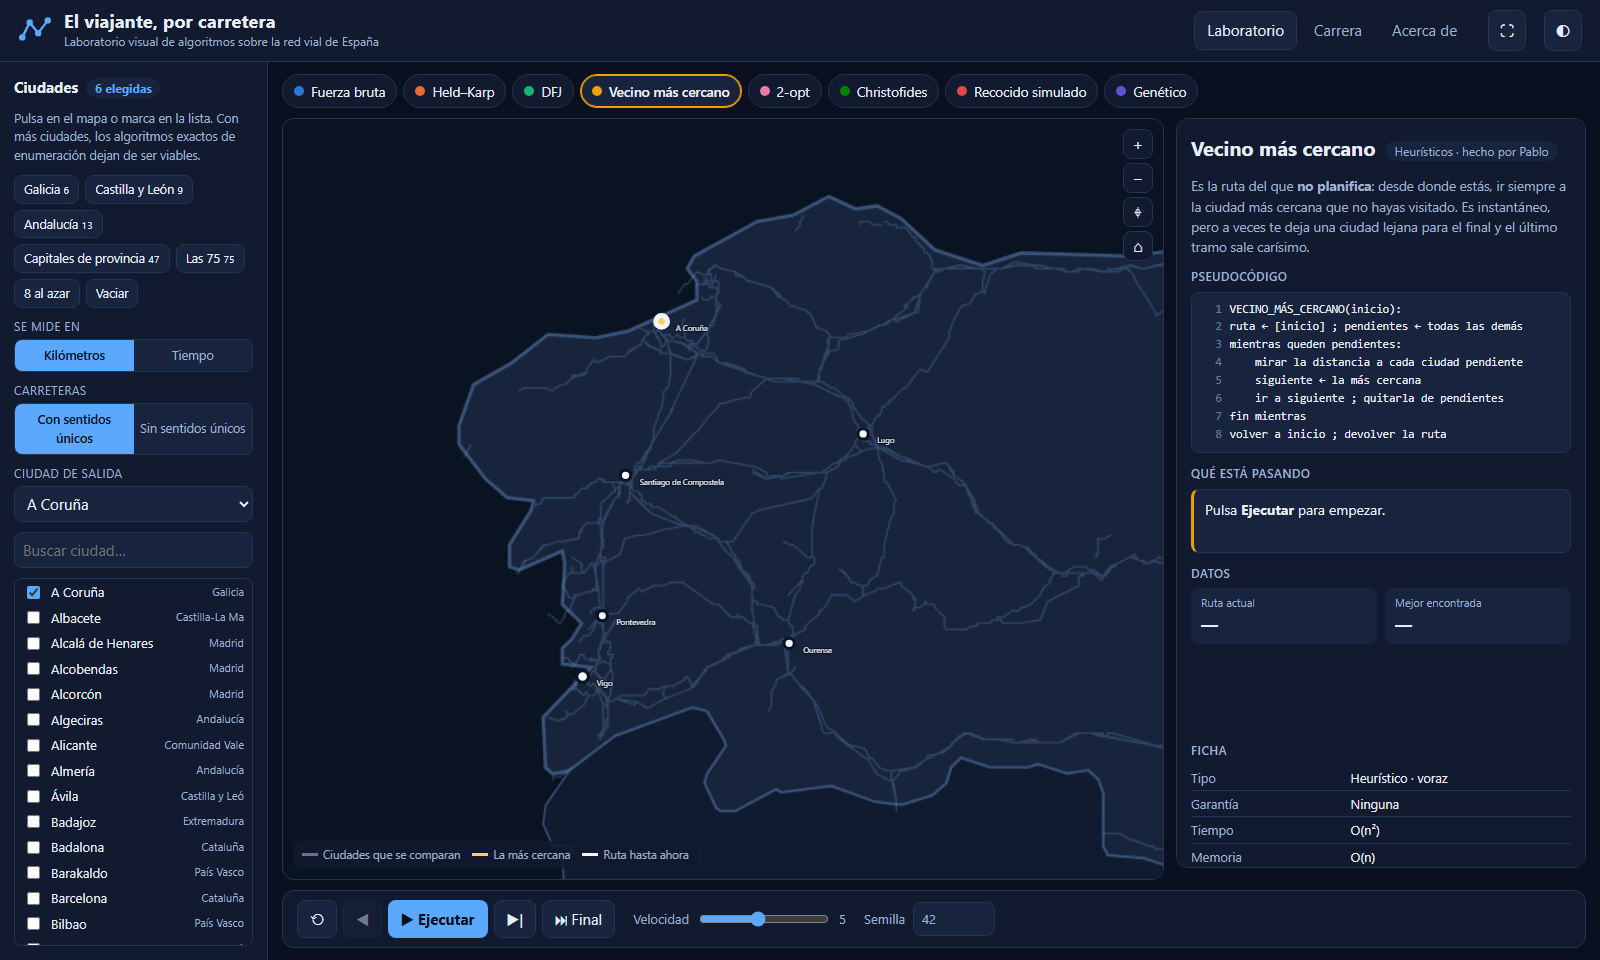
\includegraphics[width=0.97\linewidth]{01_inicio.png}
  \caption{Pantalla inicial del Laboratorio, con las 6 ciudades de Galicia y el vecino más cercano seleccionado.}
  \label{fig:g_inicio}
\end{figure}

\section{Elegir las ciudades}

\begin{itemize}
  \item \textbf{Ejemplos predefinidos} (botones de arriba del panel): \emph{Galicia} (6), \emph{Castilla y León} (9), \emph{Andalucía} (13), \emph{Capitales de provincia} (47), \emph{Las 75}, \emph{8 al azar} y \emph{Vaciar}. Al elegir un ejemplo, el mapa se acerca a las ciudades.
  \item \textbf{Pulsar sobre el mapa:} una ciudad gris se añade; una ciudad blanca se quita. También se puede marcar y desmarcar en la lista de la izquierda (con un buscador).
  \item \textbf{Ciudad de salida:} la ciudad desde la que empieza la ruta (por defecto, Madrid si está elegida).
\end{itemize}

\section{Elegir la versión del grafo}

\begin{itemize}
  \item \textbf{Se mide en: Kilómetros o Tiempo} (horas de coche). La ruta más corta no es siempre la más rápida.
  \item \textbf{Carreteras: Con sentidos únicos o Sin sentidos únicos.} Con sentidos únicos, ir de $A$ a $B$ puede costar distinto que de $B$ a $A$ (como en la realidad); sin ellos, ida y vuelta cuestan lo mismo.
\end{itemize}

\section{Controlar la ejecución}

\begin{table}[htbp]
  \centering
  \caption{Controles del reproductor.}
  \small
  \begin{tabularx}{\linewidth}{@{}l X l@{}}
    \toprule
    Botón & Qué hace & Atajo \\
    \midrule
    \textbf{Ejecutar / Pausar} & Empieza o detiene la animación (se convierte en \emph{Continuar} y, al acabar, en \emph{Repetir}). & \tecla{Espacio} \\
    \textbf{Paso} ($\blacktriangleright|$) & Avanza un solo paso. & \tecla{$\rightarrow$} \\
    \textbf{Atrás} ($\blacktriangleleft$) & Retrocede un paso. & \tecla{$\leftarrow$} \\
    \textbf{Final} & Salta directamente al resultado (en la fuerza bruta puede tardar unos segundos). & \\
    \textbf{Reiniciar} ((flecha circular)) & Vuelve al principio. & \\
    \textbf{Velocidad} & Deslizador de 1 (lento, para explicar) a 10 (muy rápido). & \\
    \textbf{Semilla} & Para el genético y el recocido: con la misma semilla repiten el mismo resultado. & \\
    \bottomrule
  \end{tabularx}
\end{table}

Además, la \textbf{rueda del ratón} hace zoom en el mapa y \textbf{arrastrar} lo mueve. Los botones de la esquina del mapa son $+$ y $-$ (zoom), $\oplus$ (encuadrar las ciudades elegidas) y $\triangle$ (ver toda la península). Arriba a la derecha hay un botón de \textbf{pantalla completa} (para presentar) y otro para cambiar entre \textbf{tema oscuro y claro}.

\section{Qué se ve con cada algoritmo}

\begin{table}[htbp]
  \centering
  \caption{Qué muestra el mapa en cada algoritmo.}
  \small
  \begin{tabularx}{\linewidth}{@{}l X@{}}
    \toprule
    Algoritmo & Qué se ve \\
    \midrule
    Fuerza bruta & Cada ruta que prueba, y un contador de rutas probadas sobre las posibles. Marca cuándo encuentra una mejor. \\
    Held--Karp & Los mejores caminos parciales por tamaño de grupo de ciudades y, al final, la ruta reconstruida hacia atrás. \\
    DFJ & La solución del problema fácil partida en \textbf{circuitos sueltos} (cada uno de un color); luego las reglas que se añaden y la solución final. \\
    Vecino más cercano & Las ciudades que compara (línea discontinua), la elegida (amarillo) y la ruta hasta ahora. \\
    2-opt & Los dos tramos que se quitan (rojo discontinuo) y los dos que se ponen (verde). \\
    Christofides & El árbol mínimo (azul), el emparejamiento (rosa) y, al final, la ruta sin repetir ciudades. \\
    Recocido simulado & La mejor ruta, la actual (tenue) y los tramos que se cambian; la temperatura baja con los niveles. \\
    Genético & La mejor ruta y 8 rutas de la población (tenues); la gráfica muestra cómo baja el coste por generación. \\
    \bottomrule
  \end{tabularx}
\end{table}

\begin{figure}[htbp]
  \centering
  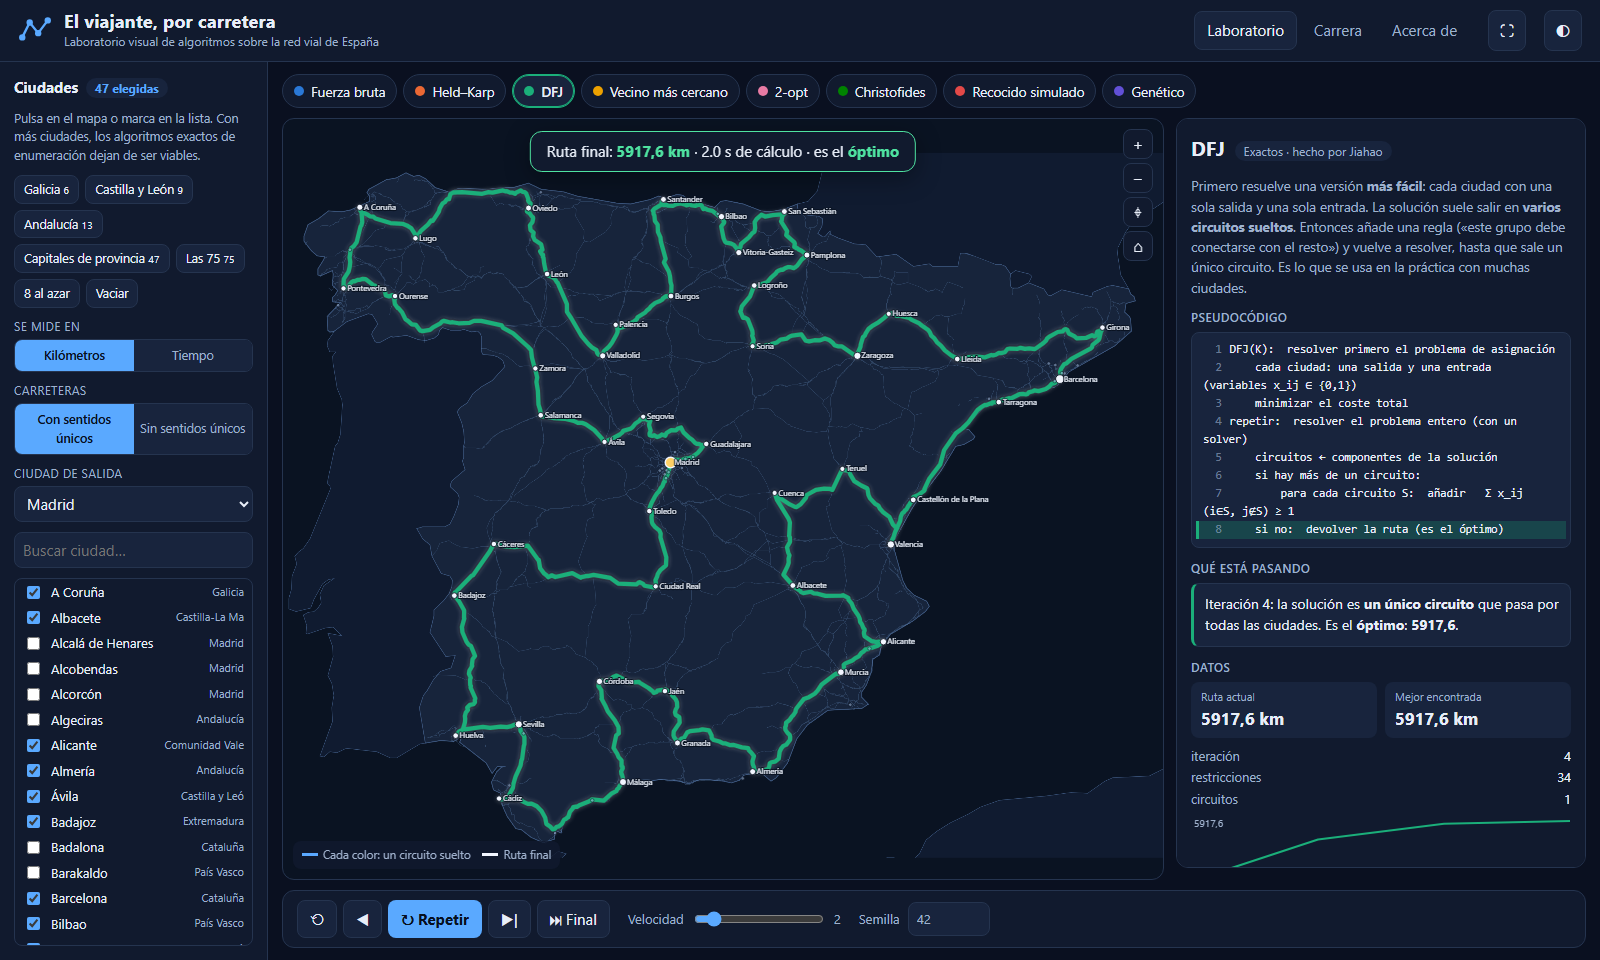
\includegraphics[width=0.97\linewidth]{06_dfj_optimo_47_capitales.png}
  \caption{Resultado final de DFJ con las 47 capitales: 5.917,6~km, el óptimo. Arriba, el cuadro con el coste y el tiempo de cálculo.}
  \label{fig:g_dfj}
\end{figure}

\section{Límites: por qué a veces no se puede ejecutar}

Algunos algoritmos no se pueden aplicar a cualquier conjunto de ciudades, y la web lo explica con un aviso amarillo (figura~\ref{fig:g_limite}). Es parte del resultado del estudio:

\begin{itemize}
  \item \textbf{Fuerza bruta:} hasta 10 ciudades en la animación. Con 47 ciudades habría $10^{58}$ rutas.
  \item \textbf{Held--Karp:} hasta 18 ciudades (su memoria se duplica con cada ciudad).
  \item \textbf{Christofides:} solo con \emph{Sin sentidos únicos}; el aviso incluye un botón para cambiarlo.
  \item Mínimo \textbf{3 ciudades} para cualquier algoritmo.
\end{itemize}

\begin{figure}[htbp]
  \centering
  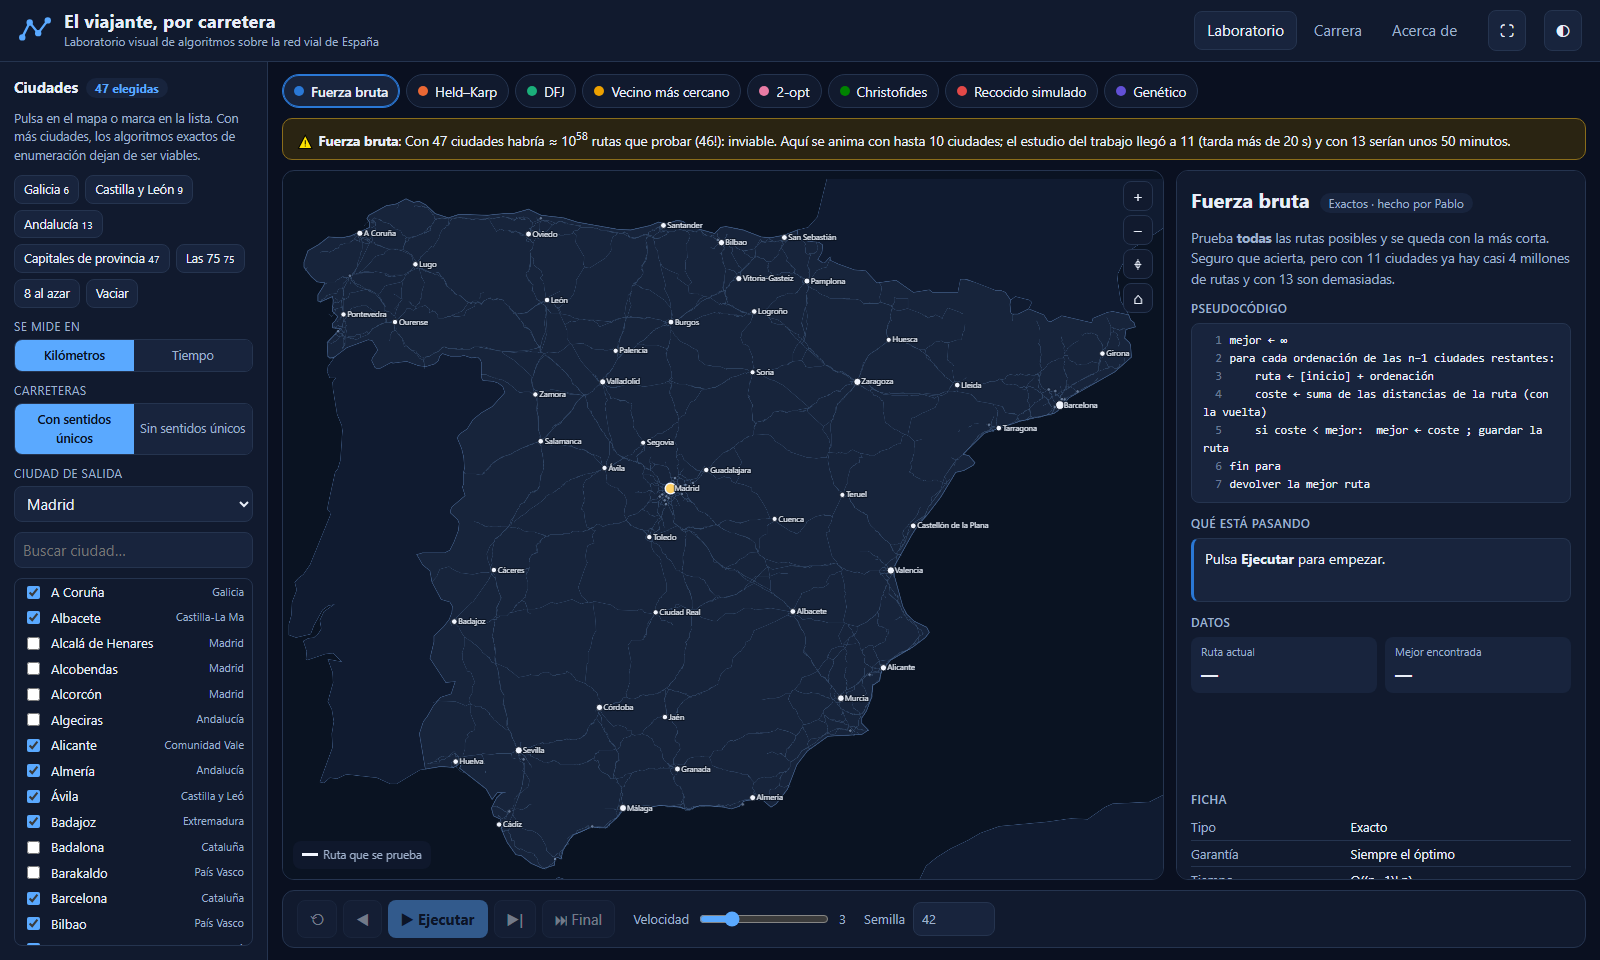
\includegraphics[width=0.97\linewidth]{09_fuerza_bruta_limite.png}
  \caption{Aviso de la fuerza bruta con las 47 capitales: explica por qué es inviable.}
  \label{fig:g_limite}
\end{figure}

\section{La pestaña Carrera}

La \emph{Carrera} pone a competir a varios algoritmos sobre \textbf{las mismas ciudades a la vez}. Se usan las ciudades y la versión elegidas en el panel izquierdo.
\begin{enumerate}[label=\textbf{\arabic*.}]
  \item Marca los algoritmos que quieres (por defecto, todos).
  \item Pulsa \textbf{¡Salida!}. Cada algoritmo avanza durante el mismo tiempo de cálculo, así que el que termina antes es el más rápido de verdad.
  \item Al terminar aparece una tabla con el coste, la desviación frente al mejor y el tiempo. un trofeo marca el mejor coste y un rayo el más rápido.
\end{enumerate}
Los algoritmos que no se pueden aplicar se muestran en gris con su motivo.

\begin{figure}[htbp]
  \centering
  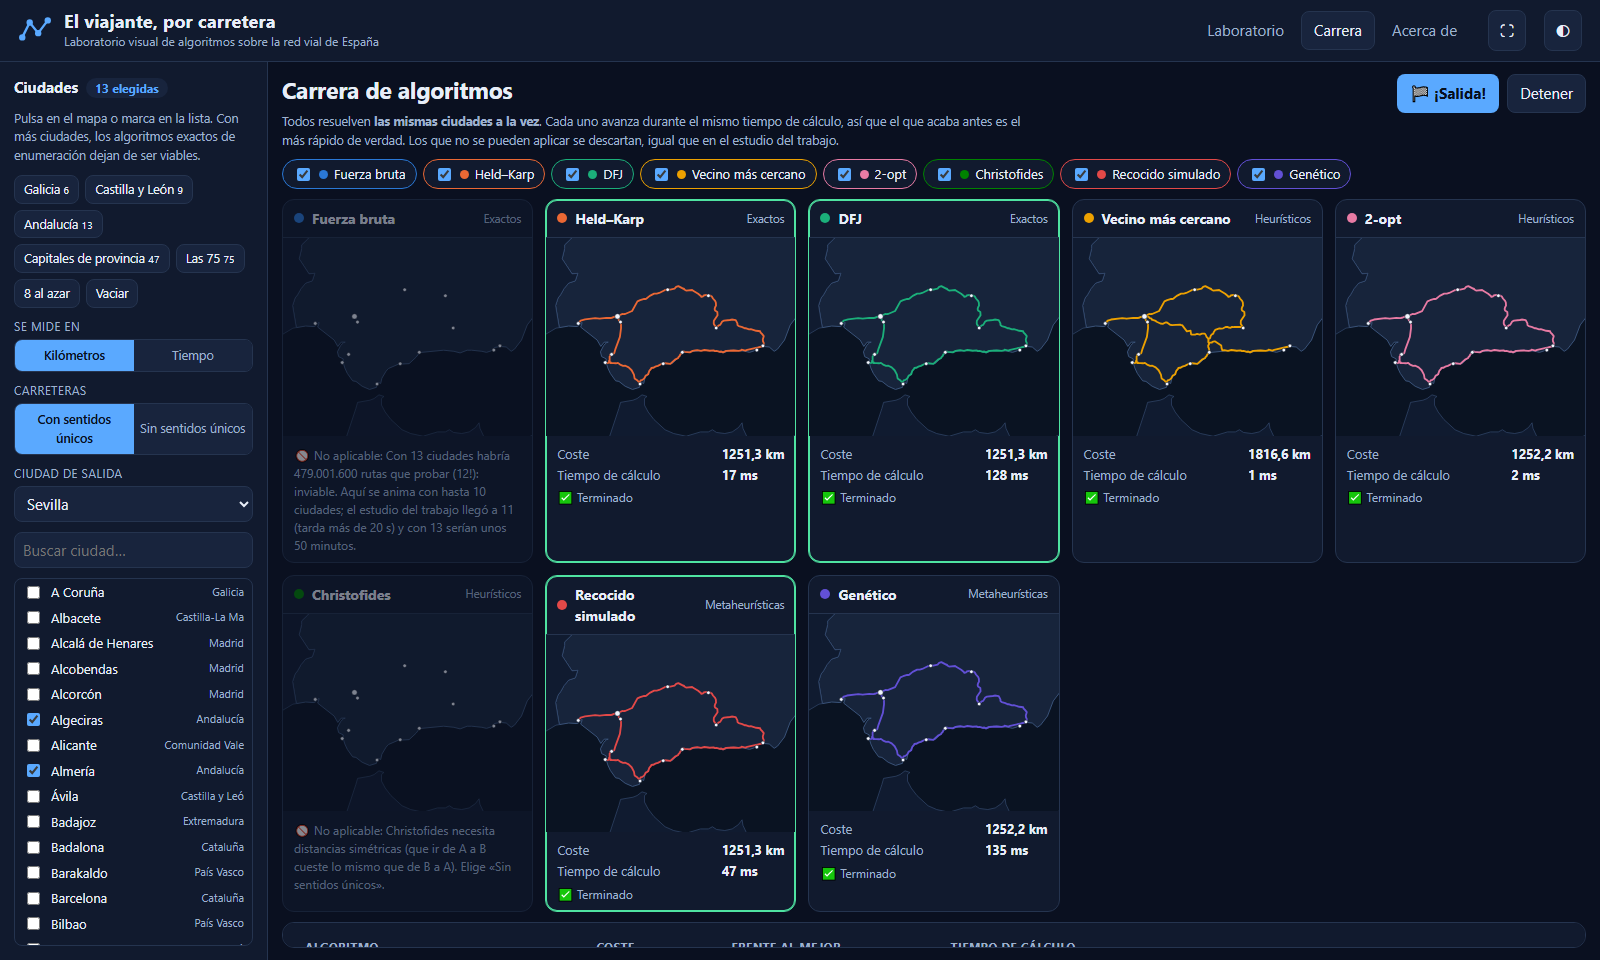
\includegraphics[width=0.97\linewidth]{10_carrera.png}
  \caption{Carrera con las 13 ciudades de Andalucía.}
  \label{fig:g_carrera}
\end{figure}

\section{Guion sugerido para la presentación}\label{g:guion}

Un recorrido de unos 6--8 minutos que cuenta la historia del trabajo (conviene pulsar el botón de pantalla completa y subir un poco el zoom del navegador):
\begin{enumerate}[label=\textbf{\arabic*.}]
  \item \textbf{El problema (1 min).} \emph{Galicia}, vecino más cercano, velocidad 3. «Un viajante, seis ciudades: ¿qué ruta?». Mostrar que la \textbf{ruta en rojo/amarillo sigue las carreteras reales}.
  \item \textbf{Fuerza bruta (1 min).} \emph{8 al azar} y \emph{Fuerza bruta}: ver cómo prueba rutas y el contador. Luego \emph{Capitales de provincia}: el aviso muestra por qué es inviable ($10^{58}$ rutas).
  \item \textbf{Mejorar sin garantías (1,5 min).} \emph{Capitales de provincia}: vecino más cercano (6.772~km) y después 2-opt, viendo cómo quita los cruces (6.326~km).
  \item \textbf{El óptimo (1,5 min).} \emph{DFJ} con las 47 capitales: los circuitos sueltos de colores, la regla que se añade y la ruta final (\textbf{5.917,6~km, el óptimo}).
  \item \textbf{Inspiración natural (1 min).} \emph{Genético} (rutas al azar que mejoran) o \emph{Recocido}.
  \item \textbf{La comparación (1,5 min).} Pestaña \emph{Carrera} con \emph{Andalucía}: Held--Karp, DFJ y recocido empatan en el óptimo; el vecino más cercano se queda un 45~\% por encima.
  \item \textbf{Conclusión.} Volver a las diapositivas: complejidad en notación $O$ y qué algoritmo usar en cada caso.
\end{enumerate}

\consejo{Antes de presentar, abre la web una vez y ejecuta DFJ: la primera vez carga el \emph{solver} (2,6~MB) y tarda un segundo más. Con el tema claro se ve mejor en una sala muy iluminada.}

\section{Publicarla en internet (GitHub Pages)}\label{g:pages}

La web \textbf{ya está publicada} en \texttt{https://raigarper.github.io/MATI\_TRABAJO/} gracias a una acción de GitHub (\emph{Publicar web}) que despliega la carpeta \texttt{web/} cada vez que cambia algo en ella y llega a la rama \texttt{main}. No hay que hacer nada: basta con hacer \emph{push}. Si hace falta lanzarla a mano, está en la pestaña \emph{Actions} del repositorio (\emph{Publicar web} y \emph{Run workflow}). Para que funcione, en \emph{Settings} y \emph{Pages} el origen (\emph{Source}) debe ser \textbf{GitHub Actions}, que es como está ahora.

% ═════════════════════════════════════════════════════════════════════
\chapter{Trabajar con los algoritmos}\label{g:algoritmos}

\section{Cómo funciona cada notebook de algoritmo}

Cada algoritmo vive en su propio \emph{notebook} dentro de \texttt{parte3/}, con el nombre \texttt{algoritmo\_autor.ipynb} (por ejemplo, \texttt{held\_karp\_raimundo.ipynb}). Todos tienen la misma estructura:
título, \textbf{ficha}, \textbf{teoría}, \textbf{código}, \textbf{pruebas} y \textbf{resultados}. Una herramienta los integra después en el \emph{notebook} principal, de modo que nadie toca \texttt{trabajo\_tsp.ipynb} y no hay conflictos de git.

El código de cada algoritmo cumple siempre el mismo \textbf{contrato}:

\begin{lstlisting}
def mi_algoritmo(K, inicio=None):
    ...
    return ruta, coste
\end{lstlisting}

\begin{itemize}
  \item \texttt{K} es el grafo de ciudades: nodos = ciudades; \texttt{K[a][b]["peso"]} es la distancia de \texttt{a} a \texttt{b} (en km u horas, según la versión). Es completo.
  \item \texttt{ruta} es la lista de \emph{todas} las ciudades, una vez cada una, en orden de visita. \texttt{coste} es el coste del ciclo \textbf{incluida la vuelta}.
  \item Debe funcionar con \texttt{K} dirigido (\texttt{nx.DiGraph}) \textbf{y} no dirigido (\texttt{nx.Graph}); si necesita simetría (como Christofides), debe avisar con un error claro.
\end{itemize}

\aviso{Dos fallos reales se descubrieron por no probar los dos tipos de grafo: el recocido simulado entraba en un bucle infinito con grafos no dirigidos y DFJ planteaba mal el modelo. Prueba siempre tu algoritmo con \texttt{general="grafo\_dirigido"} y con \texttt{general="grafo\_simple\_no\_dirigido"}.}

\section{Pasos para añadir o cambiar un algoritmo}

\begin{lstlisting}
# 1. Ponte en tu rama y trae lo ultimo
git checkout <tu-rama>
git pull origin main

# 2. Copia la plantilla con el nombre de tu algoritmo
cp parte3/_plantilla_algoritmo.ipynb parte3/<algoritmo>_<tunombre>.ipynb

# 3. Trabaja en el notebook, SOLO debajo de la linea con las tijeras
# 4. Anade tu entrada en parte3/fichas.json (copia una existente) y ejecuta:
python parte3/herramientas.py unificar

# 5. Sube tu rama
git add parte3/<algoritmo>_<tunombre>.ipynb parte3/fichas.json
git commit -m "<Algoritmo> (<tunombre>)"
git push origin <tu-rama>
\end{lstlisting}
Después, en GitHub, abre un \emph{Pull Request} de tu rama a \texttt{main}. Quien coordina lo revisa y lo acepta.

\section{Reglas}

\begin{itemize}
  \item Trabaja \textbf{siempre en tu rama}, nunca directamente en \texttt{main}, y no renombres las ramas.
  \item Un \emph{notebook} por algoritmo, con nombre \texttt{algoritmo\_autor.ipynb} en minúsculas.
  \item No edites \texttt{trabajo\_tsp.ipynb}, \texttt{data/}, \texttt{anexos/} ni la plantilla (así no hay conflictos). Si ves un error ahí, avisa.
  \item Dale a cada función un \textbf{nombre único} (\texttt{fuerza\_bruta}, \texttt{held\_karp}\dots): cuando se integren todos en un solo \emph{notebook}, los nombres no deben chocar.
  \item No crees archivos \texttt{.py} propios con el algoritmo: el código va en el \emph{notebook}. Usa solo librerías de \texttt{requirements.txt}.
  \item \textbf{Si usas IA, apunta qué le has pedido} en tu ficha y en \texttt{REGISTRO.md}.
  \item Si git avisa de un \textbf{conflicto} o algo no cuadra, no lo fuerces: avisa.
\end{itemize}

\section{Integrar los algoritmos (quien coordina)}

\begin{lstlisting}
python parte3/herramientas.py unificar    # fichas, kernel y formato estandar
python parte3/herramientas.py integrar    # copia lo que hay bajo las tijeras a la Parte 3 del notebook
\end{lstlisting}
Después se abre \texttt{trabajo\_tsp.ipynb} y se ejecuta entero (\emph{Restart \& Run All}). La herramienta es repetible: cada vez \emph{sustituye} lo integrado antes y avisa si dos \emph{notebooks} definen una función con el mismo nombre.

Si cambia el código de la Parte~2 del \emph{notebook} principal, hay que regenerar la plantilla: \texttt{python parte3/herramientas.py plantilla}.

\section{Pedir una versión del grafo}

\begin{lstlisting}
K = cargar_version(aristas="completo", nodos="capitales",
                   ambito="espana", peso="km", general="grafo_dirigido")
\end{lstlisting}

\begin{table}[htbp]
  \centering
  \caption{Parámetros de \texttt{cargar\_version}.}
  \small
  \begin{tabularx}{\linewidth}{@{}l X@{}}
    \toprule
    Parámetro & Valores \\
    \midrule
    \texttt{aristas} & \texttt{completo}, \texttt{autovias\_principales}, \texttt{solo\_autovias}, \texttt{sin\_autovias} \\
    \texttt{nodos} & \texttt{capitales} (47) o \texttt{capitales\_y\_100k} (75) \\
    \texttt{ambito} & \texttt{espana} o una comunidad: \texttt{galicia}, \texttt{andalucia}, \texttt{castilla\_y\_leon}, \texttt{cataluna}\dots \\
    \texttt{peso} & \texttt{km} o \texttt{tiempo} (en segundos) \\
    \texttt{general} & \texttt{grafo\_dirigido} o \texttt{grafo\_simple\_no\_dirigido} (los \texttt{multigrafo\_*} dan lo mismo) \\
    \bottomrule
  \end{tabularx}
\end{table}

Para probar rápido, usa una comunidad (\texttt{galicia}: 6 ciudades; \texttt{andalucia}: 13). Para un algoritmo exacto de enumeración con pocas ciudades, coge un trozo de \texttt{K} con \texttt{K.subgraph(lista\_de\_ciudades)}. Todas las versiones están en \texttt{data/versiones/catalogo.csv}.

\section{Qué escribir en tu \emph{notebook}}

Debajo de la línea de las tijeras, en este orden (borra las notas en cursiva de la plantilla cuando rellenes cada parte):
\begin{enumerate}[label=\textbf{\arabic*.}]
  \item \textbf{Teoría:} cómo funciona (en lenguaje llano y con precisión), pseudocódigo, \textbf{complejidad en tiempo y memoria} y propiedades (¿exacto?, ¿determinista?, ¿garantía?, ¿necesita simetría?, ¿hasta cuántas ciudades?).
  \item \textbf{Código:} tu función, con un comentario por bloque lógico. Si usas azar, fija una semilla.
  \item \textbf{Pruebas:} una prueba rápida con Galicia y las demás comprobaciones, con \texttt{validar\_ruta}.
  \item \textbf{Resultados:} una tabla con lo \emph{medido} (versión, ciudades, coste, tiempo, memoria). Que las cifras salgan de la ejecución, no escritas a mano.
\end{enumerate}

% ═════════════════════════════════════════════════════════════════════
\chapter{\emph{Notebook}, estudio y datos}\label{g:notebook}

\section{Las cinco partes del \emph{notebook}}

\begin{table}[htbp]
  \centering
  \caption{Partes de \texttt{trabajo\_tsp.ipynb}.}
  \small
  \begin{tabularx}{\linewidth}{@{}c l X@{}}
    \toprule
    Parte & Qué es & Necesita \\
    \midrule
    1 & Construcción del grafo (carga y dibujo) & El grafo grande (se puede saltar). \\
    2 & Versiones del grafo y \texttt{cargar\_version} & Solo \texttt{data/versiones/}. \\
    3 & Los ocho algoritmos, con pruebas y resultados & Nada más. \\
    4 & Estudio empírico (análisis y figuras) & Los CSV de \texttt{data/resultados/}. \\
    5 & Conclusiones y complejidad en notación $O$ & Nada. \\
    \bottomrule
  \end{tabularx}
\end{table}

\section{Repetir el estudio empírico}

El estudio ejecuta los ocho algoritmos sobre las 240 versiones del grafo y sobre subconjuntos de 5 a 75 ciudades. Se hace en \textbf{dos pasadas}, porque el coste de una ruta no depende de la carga del equipo pero el tiempo sí:

\begin{lstlisting}
python anexos/ejecutar_estudio.py            # en paralelo, unos 42 min (costes y calidad)
python anexos/ejecutar_estudio.py --serie    # en serie, unos 15 min (tiempos y memoria)
python anexos/ejecutar_estudio.py --prueba   # version reducida, unos minutos
\end{lstlisting}

\begin{itemize}
  \item Cada resultado se guarda al llegar: si se interrumpe, \textbf{al volver a lanzarlo reanuda} donde se quedó. \texttt{--forzar} lo repite todo desde cero.
  \item Si pasan 15 minutos sin ningún resultado nuevo, se detiene solo (algo se ha atascado).
  \item Durante la pasada \textbf{en serie}, deja el equipo en reposo y enchufado: cualquier otro programa falsea los tiempos.
\end{itemize}

Para que el \emph{notebook} vuelva a calcularlo todo, cambia \texttt{RECALCULAR\_ESTUDIO = True} en la Parte~4. Los resultados quedan en \texttt{data/resultados/} (\texttt{estudio\_resultados.csv}, \texttt{tiempos\_serie.csv}, \texttt{no\_aplicables.csv} y \texttt{calibracion.csv}).

\section{Regenerar el grafo grande}

Solo hace falta si no tienes el archivo \texttt{.graphml}:
\begin{lstlisting}
python anexos/descargar_red.py       # ~1,4 GB, ~7 min, reanudable
python anexos/construir_grafo.py     # ~4 min, ~2,3 GB de RAM
\end{lstlisting}
Si el grafo ya existe, ambos avisan y no hacen nada (\texttt{--forzar} para repetir). La web no necesita este grafo, pero si hubiera que regenerar sus datos (\texttt{web/data/}) se usa \texttt{python web/herramientas/preparar\_datos.py}, que sí lo necesita (unos 4~GB de memoria libre).

% ═════════════════════════════════════════════════════════════════════
\chapter{Compilar la memoria y esta guía}\label{g:memoria}

La memoria y esta guía están escritas en \LaTeX\ y se convierten en PDF con \textbf{Tectonic}, un compilador de un solo ejecutable que no necesita instalación y descarga los paquetes que le hacen falta.

\section{Obtener Tectonic}

Descarga el archivo para Windows (\texttt{x86\_64-pc-windows-msvc}) desde la página de versiones del proyecto (\texttt{github.com/tectonic-typesetting/tectonic/releases}), descomprímelo y deja \texttt{tectonic.exe} en una carpeta de tu elección (o en el \texttt{PATH}). Se comprueba con \texttt{tectonic --version}. En otros sistemas se puede instalar con el gestor de paquetes habitual.

\section{Compilar}

\begin{lstlisting}
# La memoria
cd memoria
tectonic -X compile memoria.tex          # genera memoria.pdf

# Esta guia
cd ../guia
tectonic -X compile guia_de_uso.tex      # genera guia_de_uso.pdf
\end{lstlisting}

La primera vez descarga paquetes y tarda un par de minutos; después es rápido. Si aparecen avisos de tipo \emph{Overfull \textbackslash hbox}, significa que alguna línea se sale del margen: conviene corregirlos.

\section{Regenerar las figuras de la memoria}

Las gráficas y mapas de la memoria salen de los resultados del estudio:
\begin{lstlisting}
python memoria/figuras/generar_figuras.py
\end{lstlisting}
Genera los PDF de \texttt{memoria/figuras/}. Si se repite el estudio, hay que regenerarlas y volver a compilar. Las capturas de pantalla de la web están en \texttt{web/capturas/}.

\section{Convenciones tipográficas}

El documento usa la fuente \emph{Libertinus} (texto y fórmulas) a 11~pt, interlineado holgado, números con coma decimal y fórmulas numeradas. Los capítulos empiezan en página nueva, y los títulos de apartado no se quedan solos al pie de página. Si añades contenido, respeta estas reglas: tablas con \texttt{tabularx} (que no se salgan del margen), figuras con \texttt{[htbp]} y fórmulas cortas.

% ═════════════════════════════════════════════════════════════════════
\chapter{Problemas frecuentes}\label{g:problemas}

\begin{table}[htbp]
  \centering
  \caption{Problemas habituales y qué hacer.}
  \small
  \begin{tabularx}{\linewidth}{@{}>{\raggedright\arraybackslash}p{0.30\linewidth} X@{}}
    \toprule
    Problema & Qué hacer \\
    \midrule
    La web sale en blanco o dice «No se han podido cargar los datos» & Se ha abierto \texttt{index.html} haciendo doble clic. Usa \texttt{iniciar\_web.bat} o \texttt{python -m http.server} desde \texttt{web/}. \\
    \texttt{python -m http.server} dice que el puerto está ocupado & Usa otro puerto: \texttt{python -m http.server 8080} y abre \texttt{http://localhost:8080}. \\
    DFJ tarda en empezar la primera vez en la web & Es normal: carga el \emph{solver} (2,6~MB). Después es inmediato. \\
    La fuerza bruta o Held--Karp no se ejecutan & El aviso amarillo explica el límite: reduce el número de ciudades. \\
    Christofides no se ejecuta & Elige «Sin sentidos únicos» (necesita distancias simétricas). \\
    El mapa se ve pequeño o desplazado & Pulsa $\oplus$ (encuadrar las ciudades) o $\triangle$ (toda la península). \\
    Error al importar \texttt{pulp} o el \emph{solver} CBC & \texttt{pip install -r requirements.txt} (instala \texttt{pulp[cbc]}). \\
    El \emph{notebook} se detiene o el equipo va lento & Falta memoria: cierra el navegador y otros programas; la Parte~1 necesita varios gigabytes. Salta la Parte~1 si no necesitas el grafo grande. \\
    Un algoritmo funciona con grafo dirigido pero falla con no dirigido & Revisa cómo lee las aristas: en un \texttt{nx.Graph} cada arista aparece \emph{una sola vez}. Convierte con \texttt{K.to\_directed()} o guarda los dos sentidos. \\
    Git dice que hay un conflicto & No lo fuerces: avisa antes de continuar. \\
    GitHub envía un correo de «Publicar web: all jobs have failed» & Mira el detalle en la pestaña \emph{Actions}. Si dice que Pages no está habilitado, el propietario debe revisar \emph{Settings}, \emph{Pages} y comprobar que el origen es GitHub Actions. \\
    Aparecen avisos \emph{Overfull \textbackslash hbox} al compilar & Una línea o tabla se sale del margen: acórtala, usa \texttt{tabularx} o permite salto de línea. \\
    \bottomrule
  \end{tabularx}
\end{table}

\section{Glosario}

\begin{description}[leftmargin=0pt,labelindent=0pt,style=nextline,itemsep=0.35em]
  \item[Grafo dirigido / no dirigido.] Con sentidos únicos, ir de $A$ a $B$ puede costar distinto que de $B$ a $A$; sin ellos, cuesta lo mismo.
  \item[Exacto.] Algoritmo que siempre encuentra la mejor ruta.
  \item[Heurística.] Método rápido que encuentra una buena ruta, pero sin garantía de que sea la mejor.
  \item[Metaheurística.] Heurística que usa el azar para explorar muchas rutas (recocido simulado, genético).
  \item[Desviación.] Cuánto por encima del óptimo queda una ruta: $(C-C^{*})/C^{*}$, en porcentaje.
  \item[Notación $O$.] Cómo crece el tiempo (o la memoria) al aumentar el número de ciudades $n$: $O(n^2)$ se multiplica por 4 al duplicar $n$; $O(2^n)$ se duplica con cada ciudad nueva.
  \item[Óptimo local.] Ruta que no se puede mejorar con pequeños cambios, aunque no sea la mejor posible.
  \item[Subciclo (circuito suelto).] En DFJ, un ciclo que no pasa por todas las ciudades y que hay que eliminar con reglas adicionales.
\end{description}

\end{document}
